\documentclass[fleqn,leqno,draft,10pt]{article}
\input{../Universidad/preamble-article.tex}

\usepackage[final]{listings} 
\lstset{
language=R, 
numbers=left, numberstyle=\tiny\ttfamily, stepnumber=2, numbersep=5pt, 
basicstyle=\ttfamily, 
stringstyle=\normalfont,
commentstyle=\itshape,
breaklines=true,
postbreak=\mbox{$\hookrightarrow$\enspace},
columns=flexible
}

\title{Notas sobre\\ análisis de datos en R}
\author{Jhonny Lanzusi}
\asignatura{Curso de edX: `Data analysis for life sciences'}

% MACROS
\newcommand{\R}{\texttt{R}} 

\begin{document}
\maketitle
\tableofcontents
\marginpar{
	\begin{abstract}
	Notas del curso de edX, algo como un resumne de lo que voy aprendiendo
	\end{abstract}
}

\section{Cosas básicas de \R}

Lo básico: operaciones, {\fontfamily{bch}\selectfont a}$a$asignación, \lstinline|for loops| y la función \lstinline|which|. 

\subsection{Operaciones básicas y asignación}%
\label{sub:operaciones_básicas_y_asignación}

En \R{} se puede operar como una simple calculadora, por ejemplo,%
\nota{La doble linea a la derecha representa bloques de código. Los \# marcan comentarios, y las lineas con \#\# marcan el resultado de ejecutar un comando}

\begin{lstlisting}
(5+27)*2
## 64
\end{lstlisting}

Los operadores aritméticos de \R\ que he usado estan en el \cref{tab:oper_arit}, y los operadores lógicos ---cuyo output es \lstinline|false| o \lstinline|true|--- estan en el \cref{tab:oper_log}.

\begin{table}\caption{Operadores aritméticos}\label{tab:oper_arit}
\begin{tabular}{rl}
	\toprule
	\texttt{+} & Suma \\
	\lstinline|-| & Resta \\
	\lstinline|*| & Multiplicación \\ 
	\lstinline|\| & División \\
	\lstinline|^| & Exponenciación. \\
	\bottomrule
\end{tabular}
\end{table}

\begin{table}\caption{Operadores Lógicos}\label{tab:oper_log}
\begin{tabular}{rl}
	\toprule
	\lstinline|>, >=| & Mayor, mayor e igual.\\
	\lstinline|<, <=| & Menor, menor e igual.\\ 
	\lstinline|=!| & No igual \\
	\lstinline.a | b. & \lstinline|True| si alguno de \lstinline|a| o \lstinline|b| es verdadero. \\
	\lstinline|a & b| & \lstinline|True| si ambos, \lstinline|a| y \lstinline|b|, son verdaderos.  \\ 
	\lstinline|isTRUE(x)| & Checkea si \lstinline|x| es verdadero.  \\
	\bottomrule
\end{tabular}
\end{table}


Como \R\ es un lenguage de programación se pueden asignar variables, por ejemplo,
\begin{lstlisting}
x <- 5+7
\end{lstlisting}
asigna el valor de \lstinline|5+7| a la variable \lstinline|x|. La asignación de puede usar con muchos tipos de elemntos en \R.

\subsection{Vectores y matrices}%
\label{sub:Vectores y matrices}

Cada vez que se da a \R\ un número, este entiende en realidad un vector con una sola componente. Para construir vectores se usa la funcion \lstinline|c()|, por ejemplo,
\begin{lstlisting}
x <- c(2.23, 3.45, 1.87, 2.11, 7.33, 18.34)
\end{lstlisting}
asigna los valores entre parénteris a la variable \lstinline|x|. 

Los vectores en \R\ pueden ser de dos tipos: atomic y lists. Los de tipo atomic son vectores en los que solo hay un tipo de datos, mientras que en las listas pueden haber tipos de datos distintos.
Los vectores atomic son los mas sencilos, sus tipos se pueden ver en el \cref{tab:vect_atom}

\begin{table}\caption{Tipos de vectores `atomic'}\label{tab:vect_atom}
\begin{tabular}{rl}
\toprule\\
numeric & Valores numéricos\\
logical & Valores del tipo TRUE y FALSE\\
character & Caracteres de texto\\
\bottomrule
\end{tabular}
\end{table}

También existe la función \lstinline|vector()| que permite crear un vector especificando su tipo (numeric, logical, etc) y despues el tamaño, por ejemplo
\begin{lstlisting}
vec1 <- vector("numeric", 100)
\end{lstlisting}
crea un vector de tipo numérico con 100 entradas, las cuales aún no estan llenas.

\subsection{Sequencias de números}%
\label{sub:Sequencias de números}

Las dos maneras mas sencillas de crear sequencias de números son la funcione \lstinline|seq| y el operador \lstinline|:|,
por ejemplo,\nota{El símbolo $\hookrightarrow$ representa la continuación de la linea anterior}
\begin{lstlisting}
1:20
## 1  2  3  4  5  6  7  8  9 10 11 12 13 14 15 16 17 18 19 20
pi:10
## 3.141593 4.141593 5.141593 6.141593 7.141593 8.141593 9.141593
15:1
## 15 14 13 12 11 10  9  8  7  6  5  4  3  2  1
\end{lstlisting}
la función \lstinline|seq| se comporta de manera similar,
\begin{lstlisting}
seq(1,20)
## 1  2  3  4  5  6  7  8  9 10 11 12 13 14 15 16 17 18 19 20
\end{lstlisting}
pero tiene mas opciones que el operador \lstinline|:|. 

La función \lstinline|rep| permite `repetir'.

\subsection{Bucles usando \lstinline|for| }%

Se pueden hacer bucles para ejercutar el mismo código varias veces, por ejemplo el siguiente código suma los cuadrados de los primeros 25 números:
\begin{lstlisting}
y <- 0

for (a in 1:25) {
  y[a] <- a^2
}
sum(y)
\end{lstlisting}

Muchos mas ejemplos de bucles se verán a lo largo de las notas.

\section{Manejo de datos}%
\label{sec:Manejo de datos}

Comenzamos leyendo un archivo con los datos y guardandolos en una variable,
\begin{lstlisting}
miceData <- read.csv("femaleMiceWeights.csv")
head(miceData)
##   Diet Bodyweight
## 1 chow      21.51
## 2 chow      28.14
## 3 chow      24.04
## 4 chow      23.45
## 5 chow      23.68
## 6 chow      19.79
\end{lstlisting}

\subsection{Introduccion a \lstinline|dplyr|}%
\label{sub:Introduccion a dplyr}


\section{Visualizacion de datos}%
\label{sec:Visualizacion}

Usaremos herramientas básicas de visualizacion de datos partiendo de \lstinline|mamsleep| (ver \cref{sub:Introduccion a dplyr}). Para darnos una idea de como luce partes de los datos, veamos un histograma del total de sueño de los mamiferos.%
\nota{La notación \lstinline|(plots[[i]] <- ...)|  puede ser ignorada con tranquilidad, es simplemente una lista que va guardando cada grafico.}
\begin{lstlisting}
library(tidyverse)
plots <- list()
mamSleep_sleep <- mamSleep$sleep_total
( plots[[1]] <- 
  ggplot(data = mamSleep, mapping = aes(x = sleep_total))+ 
  geom_histogram(binwidth = 1)
)
\end{lstlisting}

\begin{marginfigure}\caption{Total de sueño, histograma.}
	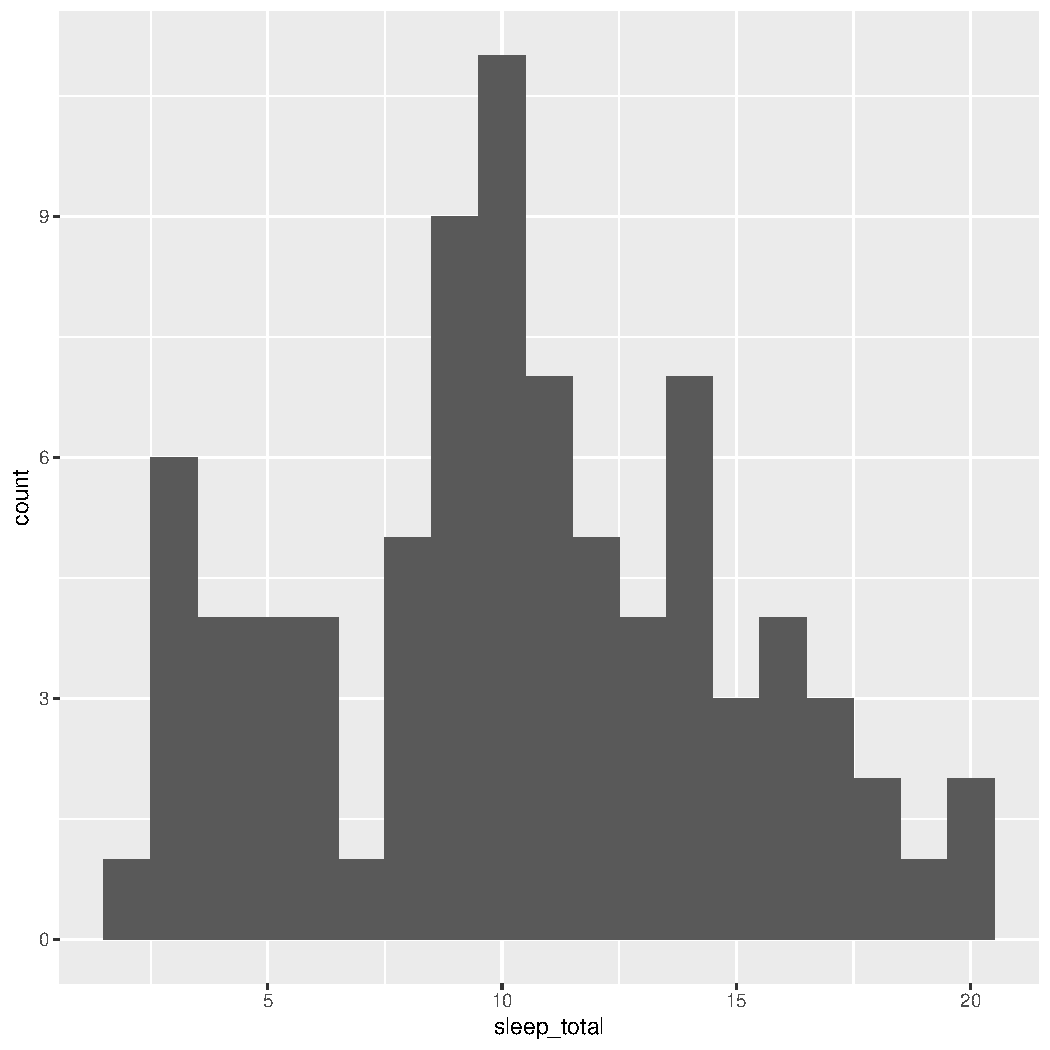
\includegraphics[width=7cm,page=1]{pics/all.pdf}	
\end{marginfigure}

\appendix
\section{Manejo de archivos}%
\label{sec:Manejo de archivos}

En \R\ se pueden manipular archivos usando funciones propias de \R, sin depender de las herramientas específicas de cada sistema operativo. Por ejemplo, la función \lstinline|getwd()| da el directorio actual.


% \printbibliography[
% heading=bibintoc,
% title={Referencias}
% ]
\end{document}
